% Created 2020-08-18 Tue 11:05
% Intended LaTeX compiler: xelatex
\documentclass[bigger,unknownkeysallowed,aspectratio=169,colorblocks]{beamer}
\usepackage{graphicx}
\usepackage{grffile}
\usepackage{minted}
\usepackage{longtable}
\usepackage{wrapfig}
\usepackage{rotating}
\usepackage[normalem]{ulem}
\usepackage{amsmath}
\usepackage{amssymb}
\usepackage{unicode-math}
\usepackage{mathtools}
\usepackage{textcomp}
\usepackage{capt-of}
\usepackage{hyperref}
\usepackage{minted}
\PassOptionsToPackage{unicode=true}{hyperref}
\PassOptionsToPackage{hyphens}{url}
\usepackage{amssymb,amsmath}
\usepackage{mathtools}
\usepackage{physics}
\usepackage{hyperref}
\hypersetup{
pdftitle={Nix Python},
pdfauthor={Rohit Goswami},
pdfborder={0 0 0},
breaklinks=true}
% Make use of float-package and set default placement for figures to H
\usepackage{float}
\floatplacement{figure}{H}
\usepackage{fontspec}
\setromanfont{EB Garamond}
\usefonttheme{serif}
\usepackage[absolute,overlay]{textpos}
\newcommand*{\XOffsetFromBottomLeft}{32.5em}%
\newcommand*{\YOffsetFromBottomLeft}{2.7ex}%
\newcommand*{\BottomLeftText}[1]{%
\par%
\scriptsize\begin{textblock*}{17.0cm}(\dimexpr\textwidth-\XOffsetFromBottomLeft\relax,\dimexpr\textheight-\YOffsetFromBottomLeft\relax)
#1%
\end{textblock*}%
}%
\usepackage[natbib]{biblatex}
\bibliography{../CarpentryCon2020.bib}
\usetheme{Verona}
\author{Rohit and Amrita Goswami}
\date{\today}
\title{Nix Python}
\subtitle{Fundamentals and Rationale}
\titlegraphic[scale=0.6]{images/carpen2020.png}{}
\institute{Presented at \textbf{CarpentryCon 2020}}
\mail{rog32@hi.is}
\hypersetup{
 pdfauthor={Rohit and Amrita Goswami},
 pdftitle={Nix Python},
 pdfkeywords={},
 pdfsubject={},
 pdfcreator={Emacs 27.1 (Org mode 9.4)}, 
 pdflang={English}}
\begin{document}

\maketitle

\begin{frame}[label={sec:org12a81ce},fragile]{Python Modules}
 \begin{itemize}
\item A \texttt{.py} file is a \alert{module}
\item It is \alert{standalone} if it only imports from the standard library
\end{itemize}
\end{frame}
\begin{frame}[label={sec:orgb8270dd},fragile]{Pure Python Packages}
 \begin{itemize}
\item A directory with \texttt{\_\_init\_\_.py} in it is a \alert{package}
\item Use \texttt{pip}
\end{itemize}
\end{frame}
\begin{frame}[label={sec:org82c0bf9},fragile]{More Distributions}
 \begin{itemize}
\item Distributions have zero or more packages
\item Built by \texttt{setuptools} with \texttt{setup.py}
\item Simple source only \texttt{.tar.gz}
\end{itemize}
\end{frame}
\begin{frame}[label={sec:org0ee7dea}]{The Python Gradient}
From here: \url{https://www.youtube.com/watch?v=iLVNWfPWAC8}

\begin{center}
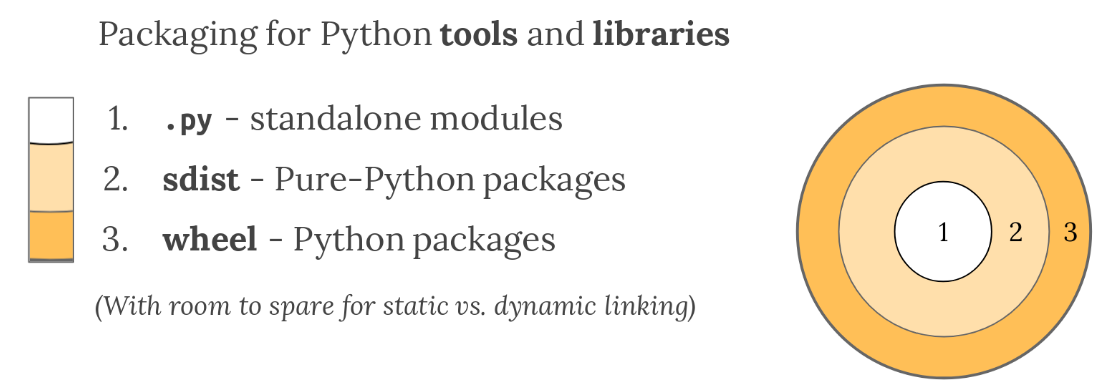
\includegraphics[width=.9\linewidth]{images/The_Python_Gradient/2020-05-22_23-00-30_screenshot.png}
\end{center}
\begin{itemize}
\item Libraries and Dev tools are all we get (from PyPI)
\end{itemize}
\end{frame}
\begin{frame}[label={sec:orgaa53f83}]{Pip Requirements}
\begin{itemize}
\item Python
\item System libraries
\item Build tools
\begin{itemize}
\item Wheels don't work for arbitrary distributions
\end{itemize}
\end{itemize}
\end{frame}
\begin{frame}[label={sec:orgd496c8b}]{What?}
\begin{center}
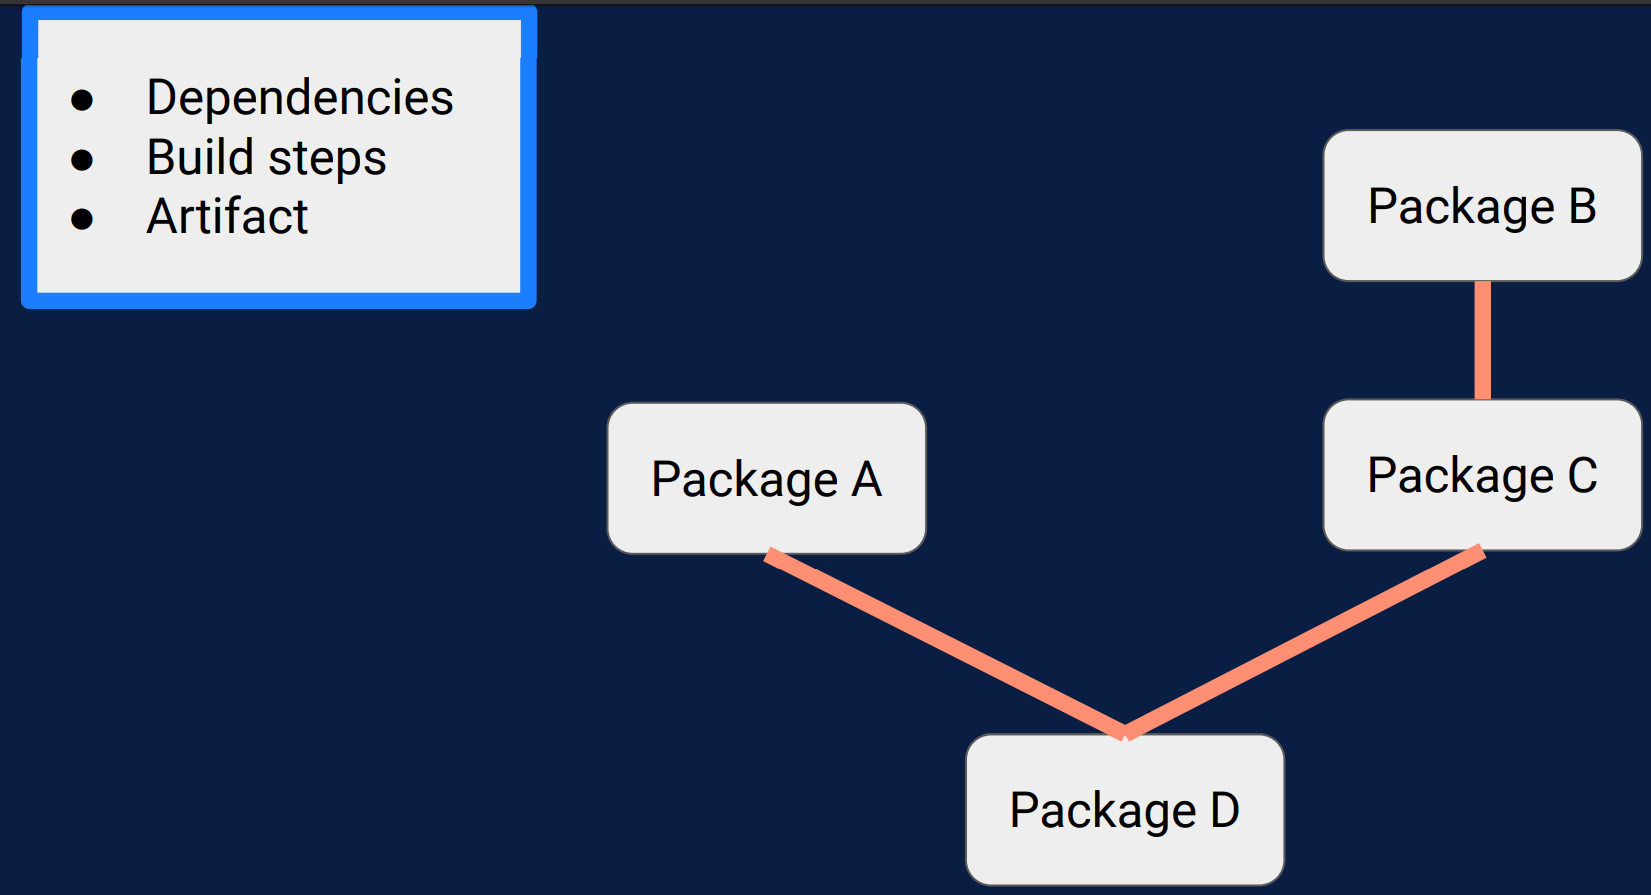
\includegraphics[width=0.5\linewidth]{images/What?/2020-05-22_23-04-53_screenshot.png}
\end{center}
\begin{itemize}
\item \tiny from \url{https://brianmckenna.org/files/presentations/rootconf19-nix.pdf}
\end{itemize}
\end{frame}
\begin{frame}[label={sec:org50be56b}]{Nix}
\begin{columns}
\begin{column}{0.4\columnwidth}
\fullcite{dolstraNixSafePolicyFree2004,dolstraNixOSPurelyFunctional2010}
\end{column}
\begin{column}{0.6\columnwidth}
\begin{center}
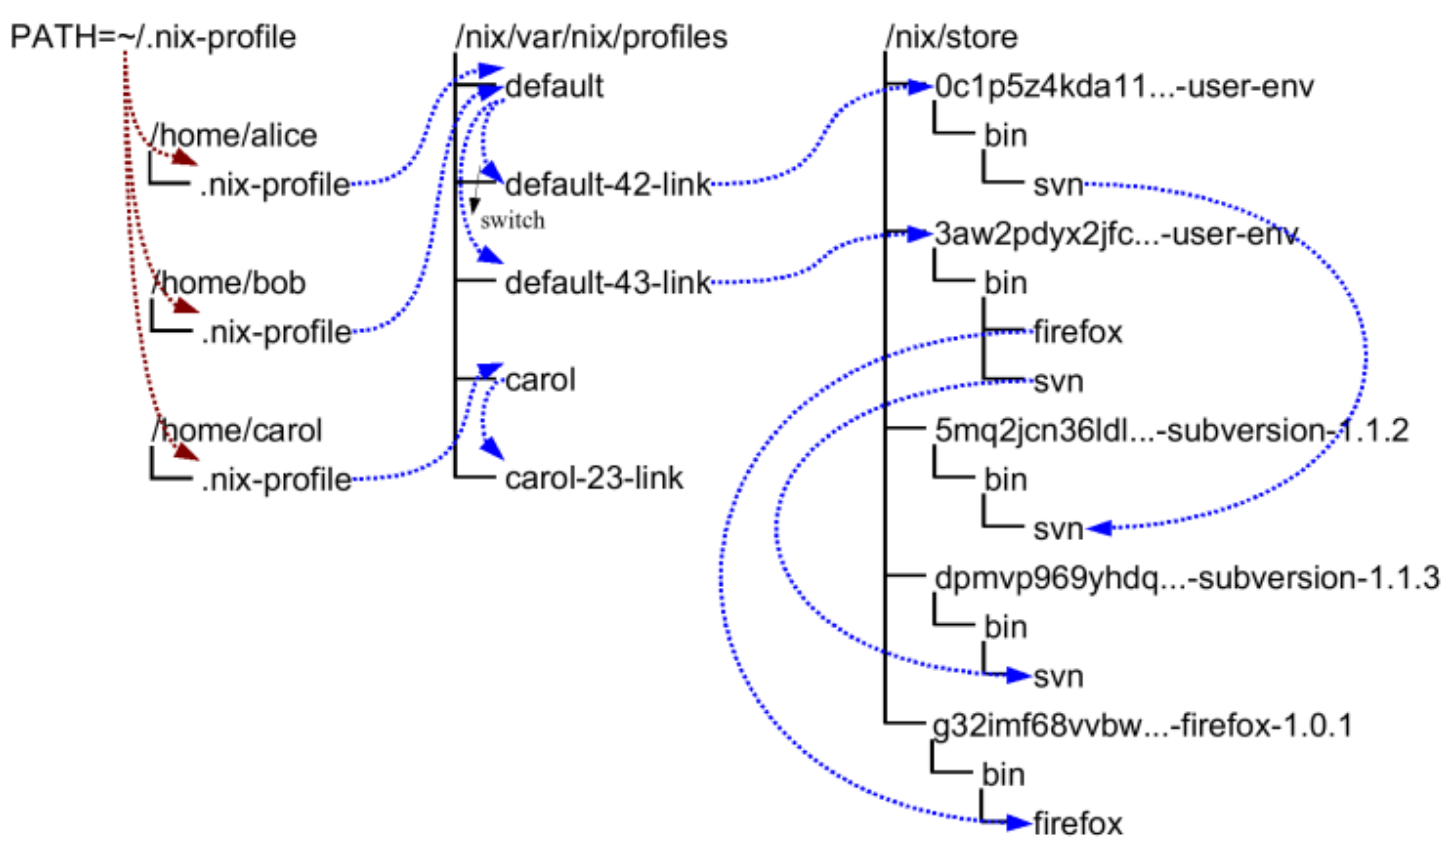
\includegraphics[width=.9\linewidth]{images/A_screenshot/2020-05-22_23-15-22_screenshot.png}
\end{center}
\end{column}
\end{columns}
\end{frame}
\begin{frame}[label={sec:org5e350d2}]{Why?}
\begin{columns}
\begin{column}{0.4\columnwidth}
\begin{quote}
Protects against self harm
\end{quote}
\begin{quote}
Exposes things taken for granted
\end{quote}
\begin{quote}
Enforces consistency
\end{quote}
\end{column}
\begin{column}{0.6\columnwidth}
\begin{description}
\item[{Reliable}] Purely functional, no broken dependencies
\item[{Reproducible}] Each package is in isolation
\item[{How?}] store + hash + name + version
\end{description}
\end{column}
\end{columns}
\end{frame}
\begin{frame}[label={sec:org2c2749e},fragile]{Installation (Multi-User)}
 \begin{minted}[bgcolor=white,breaklines=true,linenos=true,style=tango]{bash}
sh <(curl https://nixos.org/nix/install) --daemon
\end{minted}
\begin{itemize}
\item Needs \texttt{sudo} but should not be run as root
\item Will make build users with IDs between 30001 and 30032 along with a group ID 30000
\end{itemize}
\end{frame}
\begin{frame}[label={sec:orga5c7edc},fragile]{Nix Python - Trial I}
 \begin{minted}[bgcolor=white,breaklines=true,linenos=true,style=tango]{bash}
nix-shell -p 'python38.withPackages(ps: with ps; [ numpy toolz ])'
\end{minted}

\begin{itemize}
\item Check which \texttt{python} is loaded
\item Check which modules are present
\end{itemize}
\end{frame}
\begin{frame}[label={sec:org4fe563a},fragile]{Shell in a File}
 \begin{columns}
\begin{column}{0.6\columnwidth}
\begin{minted}[bgcolor=white,breaklines=true,linenos=true,style=tango]{nix}
with import <nixpkgs> {};

let
  pythonEnv = python35.withPackages (ps: [
    ps.numpy
    ps.toolz
  ]);
in mkShell {
  buildInputs = [
    pythonEnv
    which
  ];
}
\end{minted}
\end{column}
\begin{column}{0.4\columnwidth}
\begin{itemize}
\item What \alert{tools} are we adding?
\item What \alert{environment} are we using?
\end{itemize}
\end{column}
\end{columns}
\end{frame}
\begin{frame}[label={sec:org9324ad5},fragile]{An Aside into Purity}
 \begin{columns}
\begin{column}{0.4\columnwidth}
\begin{minted}[bgcolor=white,breaklines=true,linenos=true,style=tango]{bash}
nix-shell --pure --run 'bash'
\end{minted}
\begin{itemize}
\item Why?
\item What do we solve with this?
\end{itemize}
\end{column}

\begin{column}{0.6\columnwidth}
\begin{figure}[htbp]
\centering
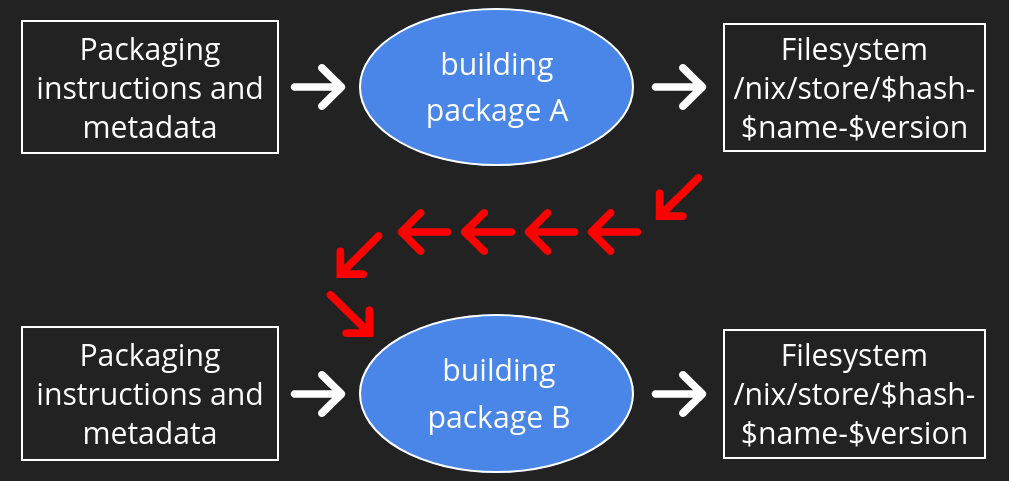
\includegraphics[width=.9\linewidth]{images/A_screenshot/2020-05-22_23-57-17_screenshot.png}
\caption{Stateless builds from \url{https://slides.com/garbas/mozilla-all-hands-london-2016\#/7/0/3}}
\end{figure}
\end{column}
\end{columns}
\end{frame}

\begin{frame}[label={sec:org2cacc75},fragile]{Nix with Scripts}
 \begin{minted}[bgcolor=white,breaklines=true,linenos=true,style=tango]{bash}
#! /usr/bin/env nix-shell
#! nix-shell -i python3 -p "python3.withPackages(ps: [ps.numpy])"

import numpy

print(numpy.__version__)
\end{minted}
\end{frame}
\begin{frame}[label={sec:orgd2ec866},fragile]{Friendly Nix}
 \begin{columns}
\begin{column}{0.4\columnwidth}
\begin{minted}[bgcolor=white,breaklines=true,linenos=true,style=tango]{bash}
nix-env -i nox
nox niv
\end{minted}
\end{column}
\begin{column}{0.6\columnwidth}
\begin{description}
\item[{Niv}] For pinning packages
\item[{Nox}] Interactive package management
\item[{\href{https://github.com/target/lorri/}{Lorri}}] For automatically reloading environments
\end{description}
\end{column}
\end{columns}
\end{frame}
\begin{frame}[label={sec:orgad987dd}]{Existing Projects?}
\begin{columns}
\begin{column}{0.4\columnwidth}
\begin{description}
\item[{Pip}] pip2nix
\item[{Poetry}] poetry2nix
\item[{Anaconda/Miniconda}] Why? -\_-
\item[{Virtualenv}] \ldots{}
\end{description}
\end{column}
\begin{column}{0.6\columnwidth}
\begin{figure}[htbp]
\centering
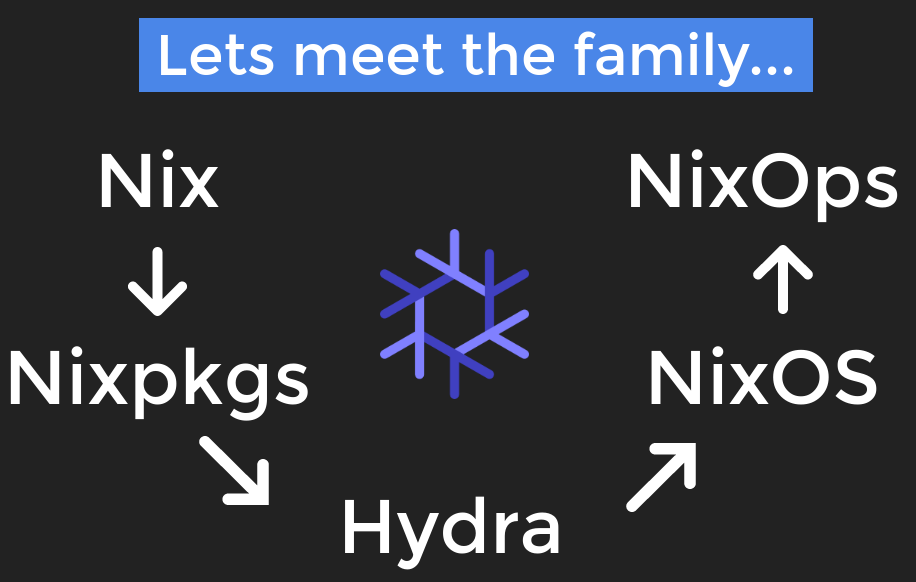
\includegraphics[width=.9\linewidth]{images/A_screenshot/2020-05-22_23-55-07_screenshot.png}
\caption{From \url{https://slides.com/garbas/mozilla-all-hands-london-2016\#/8/0/8}}
\end{figure}
\end{column}
\end{columns}
\end{frame}

\begin{frame}[label={sec:org35065dd}]{Future Directions!}
\begin{columns}
\begin{column}{0.6\columnwidth}
\begin{itemize}
\item Read up on the Python Guide
\item Try \href{https://nixos.org/nixos/nix-pills/why-you-should-give-it-a-try.html}{Nix Pills}
\item Roll your own environment
\item Make a docker image
\item Try a more \href{https://github.com/d-SEAMS/seams-core/blob/691da72262db40625774a2aed05d23c17a211360/nix/pkgs/sharkML/sharkML.nix}{complex system} (\href{https://dseams.info}{d-SEAMS} \cite{goswamiDSEAMSDeferredStructural2020})
\end{itemize}
\end{column}
\begin{column}{0.4\columnwidth}
\begin{center}
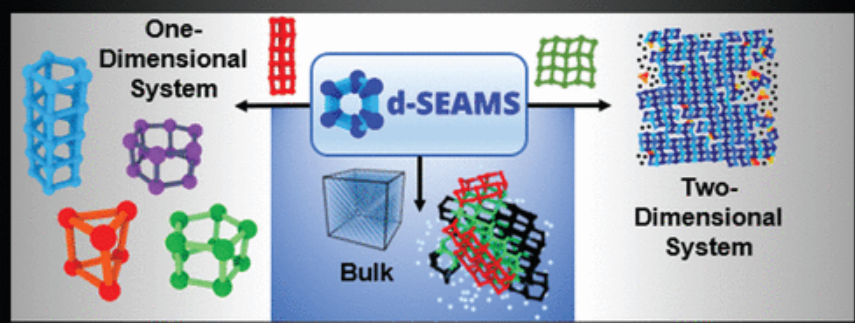
\includegraphics[width=.9\linewidth]{images/A_screenshot/2020-05-22_23-54-29_screenshot.png}
\end{center}
\end{column}
\end{columns}
\end{frame}

\begin{frame}[allowframebreaks]{References}
\printbibliography
\end{frame}

\begin{frame}[label={sec:org5b016d4},standout]{End}
\begin{center}
\Huge Thank you
\end{center}
\end{frame}
\end{document}
